\documentclass[12pt]{article}
	
\usepackage[margin=1in]{geometry}		% For setting margins
\usepackage{amsmath}				% For Math
\usepackage{fancyhdr}				% For fancy header/footer
\usepackage{graphicx}				% For including figure/image
\usepackage{cancel}					% To use the slash to cancel out stuff in work

%%%%%%%%%%%%%%%%%%%%%%
% Set up fancy header/footer
\pagestyle{fancy}
\fancyhead[LO,L]{Jennifer Byford}
\fancyhead[CO,C]{ECE305 - Homework Example}
\fancyhead[RO,R]{\today}
\fancyfoot[LO,L]{}
\fancyfoot[CO,C]{\thepage}
\fancyfoot[RO,R]{}
\renewcommand{\headrulewidth}{0.4pt}
\renewcommand{\footrulewidth}{0.4pt}
%%%%%%%%%%%%%%%%%%%%%%

\begin{document}
\noindent \textit{A uniformly charged dielectric gel having charge density $\rho_v = \rho_o$ and dielectric constant of $\epsilon_r = 2$ is enclosed inside a dielectric shell with dielectric constant of $\epsilon_r = 5$ as shown in the figure. The dielectric shell is surrounded by free space ($\epsilon_r = 1$). Determine E, $\Phi$, D, P in all regions.}

\begin{figure}[!h] 
	\begin{centering}
		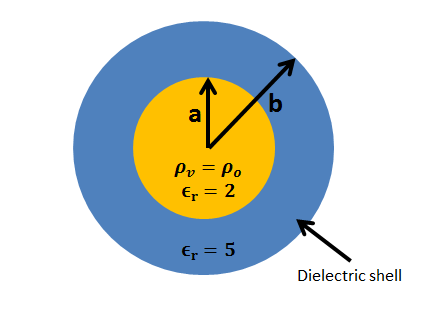
\includegraphics[keepaspectratio = true, width = 2in]{image.PNG}
		\caption{Given scenario.}
	\end{centering}
\end{figure}

\noindent In this problem we can consider there to be 3 regions, (1)~$r < a$, (2)~$a \leq r < b$, and (3)~$r \geq b$. For finding the electric flux density Gauss's Law provides the most straight forward solution. Then, using the constitutive relation between electric flux density and electric field, $\vec{E}$ can be found. Thereafter $\vec{P}$ and $\Phi$ are directly related to $\vec{E}$.\\
\\
\underline{Electric Flux Density:}
	\begin{align*}
		\oint_S \vec{D} \cdot \hat{n} &= Q_{en} \\
		\int_0^\pi \int_0^{2\pi} D_r r^2 sin\theta d\phi d\theta &= Q_{en}\\	
		4\pi r^2 D_r &= Q_{en}
	\end{align*}

\textit{Region 1}			
	\begin{align*}
		Q_{en} &= \int_0^\pi \int_0^{2\pi} \int_0^r \rho_o r^2 sin\theta dr d\phi d\theta \\	
		Q_{en} &= \frac{4\pi \rho_o r^3}{3} \\
		4\pi r^2 D_r &= \frac{4\pi \rho_o r^3}{3} \\
		\vec{D} &= \frac{\rho_o r^3}{3 r^2} \\
		\vec{D} &= \frac{\rho_o r}{3} \hat{r}~C/m^2
	\end{align*}
	
\textit{Region 2 and 3}			
	\begin{align*}
		Q_{en} &= \int_0^\pi \int_0^{2\pi} \int_0^a \rho_o r^2 sin\theta dr d\phi d\theta \\	
		Q_{en} &= \frac{4\pi \rho_o a^3}{3} \\
		4\pi r^2 D_r &= \frac{4\pi \rho_o a^3}{3} \\
		\vec{D} &= \frac{\rho_o a^3}{3 r^2} \hat{r}~C/m^2
	\end{align*}
		
\underline{Electric Field:}
	\begin{align*}
		\vec{D} &= \epsilon \vec{E} \\
		\vec{E} &= \frac{1}{\epsilon} \vec{D} \\
		\vec{E} &= \frac{1}{\epsilon_o \epsilon_r} \vec{D}
	\end{align*}
	
\textit{Region 1}			
	\begin{align*}
		\vec{E} &= \frac{1}{\epsilon_o \epsilon_r} \vec{D} \\
		\vec{E} &= \frac{1}{\epsilon_o \epsilon_r} \frac{\rho_o r}{3} \\
		\vec{E} &= \frac{1}{2 \epsilon_o} \frac{\rho_o r}{3} \hat{r}~V/m
	\end{align*}
	
\textit{Region 2}			
	\begin{align*}
		\vec{E} &= \frac{1}{\epsilon_o \epsilon_r} \vec{D} \\
		\vec{E} &= \frac{1}{\epsilon_o \epsilon_r} \frac{\rho_o a^3}{3 r^2} \\
		\vec{E} &= \frac{1}{5 \epsilon_o} \frac{\rho_o a^3}{3 r^2} \hat{r}~V/m
	\end{align*}
	
\textit{Region 3}			
	\begin{align*}
		\vec{E} &= \frac{1}{\epsilon_o \epsilon_r} \vec{D} \\
		\vec{E} &= \frac{1}{\epsilon_o \epsilon_r} \frac{\rho_o a^3}{3 r^2} \\
		\vec{E} &= \frac{1}{\epsilon_o} \frac{\rho_o a^3}{3 r^2} \hat{r}~V/m
	\end{align*}
		
\underline{Electric Polarization:}
	$$\vec{P} = (\epsilon_r - 1)\epsilon_o \vec{E}$$
	
\textit{Region 1}			
	\begin{align*}
		\vec{P} &= (\epsilon_r - 1)\epsilon_o \vec{E} \\
		\vec{P} &= (2 - 1) \cancel{\epsilon_o} \frac{1}{2 \cancel{\epsilon_o}} \frac{\rho_o r}{3} \\
		\vec{P} &= \frac{1}{2} \frac{\rho_o r}{3} \\
		\vec{P} &= \frac{\rho_o r}{6} \hat{r}~C/m^2
	\end{align*}
	
\textit{Region 2}			
	\begin{align*}
		\vec{P} &= (\epsilon_r - 1)\epsilon_o \vec{E} \\
		\vec{P} &= (5 - 1) \cancel{\epsilon_o} \frac{1}{5 \cancel{\epsilon_o}} \frac{\rho_o a^3}{3 r^2} \\
		\vec{P} &= \frac{4}{5} \frac{\rho_o a^3}{3 r^2}\\
		\vec{P} &= \frac{4\rho_o a^3}{15 r^2} \hat{r}~C/m^2
	\end{align*}
	
\textit{Region 3}			
	\begin{align*}
		\vec{P} &= (\epsilon_r - 1)\epsilon_o \vec{E} \\
		\vec{P} &= (1 - 1) \epsilon_o \vec{E} \\
		\vec{P} &= 0 \hat{r}~C/m^2
	\end{align*}
		
\underline{Electric Potential:}

	$$\Phi = -\int_{\infty}^{r} \vec{E} \cdot dl$$
	
	% e region 1 = \frac{1}{2 \epsilon_o} \frac{\rho_o r}{3} \hat{r}
	% e region 2  = \frac{1}{5 \epsilon_o} \frac{\rho_o a^3}{3 r^2} \hat{r}
	% e region 3 = \frac{1}{\epsilon_o} \frac{\rho_o a^3}{3 r^2} \hat{r}
	
\textit{Region 3}			
	\begin{align*}
		\Phi &= -\int_{\infty}^{r} \vec{E}_3 \cdot dl \\
		\Phi &= -\int_{\infty}^{r} \frac{1}{\epsilon_o} \frac{\rho_o a^3}{3 r^2} \hat{r} \cdot \hat{r} dr \\
		\Phi &= -\frac{\rho_o a^3}{3 \epsilon_o} \int_{\infty}^{r} \frac{1}{r^2} dr \\
		\Phi &= -\frac{\rho_o a^3}{3 \epsilon_o} \left[-\frac{1}{r}\right]_\infty^r \\
		\Phi &= \frac{\rho_o a^3}{3\epsilon_o r} \\
		\Phi &= \frac{\rho_o a^3}{3\epsilon_o r}~V
	\end{align*}
		
\textit{Region 2}
	\begin{align*}
		\Phi &= -\int_{\infty}^{r} \vec{E} \cdot dl \\
		\Phi &= -\int_{\infty}^{b} \vec{E}_3 \cdot dl - \int_b^r \vec{E}_2 \cdot dl\\
		\Phi &= -\int_{\infty}^{b} \frac{1}{\epsilon_o} \frac{\rho_o a^3}{3 r^2} \hat{r} \cdot \hat{r} dr - \int_b^r \frac{1}{5 \epsilon_o} \frac{\rho_o a^3}{3 r^2} \hat{r} \cdot \hat{r} dr\\
		\Phi &= -\frac{\rho_o a^3}{3 \epsilon_o} \int_{\infty}^{b} \frac{1}{r^2} dr - \frac{\rho_o a^3}{15 \epsilon_o} \int_b^r \frac{1}{r^2} dr\\
		\Phi &= -\frac{\rho_o a^3}{3 \epsilon_o} \left[-\frac{1}{r}\right]_\infty^b - \frac{\rho_o a^3}{15 \epsilon_o} \left[-\frac{1}{r}\right]_b^r\\
		\Phi &= \frac{\rho_o a^3}{3 \epsilon_o} \frac{1}{b} + \frac{\rho_o a^3}{15 \epsilon_o} \left[\frac{1}{r} - \frac{1}{b}\right]\\
		\Phi &= \frac{\rho_o a^3}{3 \epsilon_o b} + \frac{\rho_o a^3}{15 \epsilon_o r} - \frac{\rho_o a^3}{15 \epsilon_o b}~V
	\end{align*}

	
\textit{Region 1}	
	\begin{align*}
		\Phi &= -\int_{\infty}^{r} \vec{E} \cdot dl \\
		\Phi &= -\int_{\infty}^{b} \vec{E}_3 \cdot dl - \int_b^a \vec{E}_2 \cdot dl - \int_a^r \vec{E}_1 \cdot dl\\
		\Phi &= -\int_{\infty}^{b} \frac{1}{\epsilon_o} \frac{\rho_o a^3}{3 r^2} \hat{r} \cdot \hat{r} dr - \int_b^a \frac{1}{5 \epsilon_o} \frac{\rho_o a^3}{3 r^2} \hat{r} \cdot \hat{r} dr - \int_a^r \frac{1}{2 \epsilon_o} \frac{\rho_o r}{3} \hat{r} \cdot \hat{r} dr\\
		\Phi &= -\frac{\rho_o a^3}{3 \epsilon_o} \int_{\infty}^{b} \frac{1}{r^2} dr - \frac{\rho_o a^3}{15 \epsilon_o} \int_b^a \frac{1}{r^2} dr  - \frac{\rho_o}{6 \epsilon_o} \int_a^r r dr\\
		\Phi &= -\frac{\rho_o a^3}{3 \epsilon_o} \left[-\frac{1}{r}\right]_\infty^b - \frac{\rho_o a^3}{15 \epsilon_o} \left[-\frac{1}{r}\right]_b^a - \frac{\rho_o}{6 \epsilon_o} \left[\frac{r^2}{2}\right]_a^r\\
		\Phi &= \frac{\rho_o a^3}{3 \epsilon_o} \frac{1}{b} + \frac{\rho_o a^3}{15 \epsilon_o} \left[\frac{1}{a} - \frac{1}{b}\right] - \frac{\rho_o}{12 \epsilon_o} \left[r^2 - a^2\right]\\
		\Phi &= \frac{\rho_o a^3}{3 \epsilon_o b} + \frac{\rho_o a^3}{15 \epsilon_o a} - \frac{\rho_o a^3}{15 \epsilon_o b} - \frac{\rho_o r^2}{12 \epsilon_o} + \frac{\rho_o a^2}{12 \epsilon_o}\\
		\Phi &= \frac{\rho_o a^3}{3 \epsilon_o b} + \frac{\rho_o a^2}{15 \epsilon_o} - \frac{\rho_o a^3}{15 \epsilon_o b} - \frac{\rho_o r^2}{12 \epsilon_o} + \frac{\rho_o a^2}{12 \epsilon_o}\\
		\Phi &= \frac{\rho_o a^2}{\epsilon_o}\left[ \frac{a}{3b} + \frac{1}{15} + \frac{1}{12}\right] - \frac{\rho_o}{\epsilon_o}\left[\frac{a^3}{15b} + \frac{r^2}{12}\right]~V
	\end{align*}		

		
Final Answer Summary:
		
\begin{tabular}{| c | c | c | c |}
\hline
& Region 1 ($r<a$)& Region 2 ($a\leq r < b$)& Region 3 ($r\geq b$)\\ \hline
$\vec{D}~(C/m^2)$ & $\frac{\rho_o r}{3} \hat{r}$ & $\frac{\rho_o a^3}{3 r^2} \hat{r}$ & $\frac{\rho_o a^3}{3 r^2} \hat{r}$\\
$\vec{E}~(V/m)$ & $\frac{\rho_o r}{6 \epsilon_o} \hat{r}$ & $\frac{1}{5 \epsilon_o} \frac{\rho_o a^3}{3 r^2} \hat{r}$ & $\frac{1}{\epsilon_o} \frac{\rho_o a^3}{3 r^2} \hat{r}$\\
$\vec{P}~(C/m^2)$ & $\frac{\rho_o r}{6} \hat{r}$ & $\frac{4\rho_o a^3}{15 r^2} \hat{r}$ & $0 \hat{r}$\\
$\Phi~(V)$ &  $\frac{\rho_o a^2}{\epsilon_o}\left[ \frac{a}{3b} + \frac{1}{15} + \frac{1}{12}\right] - \frac{\rho_o}{\epsilon_o}\left[\frac{a^3}{15b} + \frac{r^2}{12}\right]$ & $\frac{\rho_o a^3}{3 \epsilon_o b} + \frac{\rho_o a^3}{15 \epsilon_o r} - \frac{\rho_o a^3}{15 \epsilon_o b}$ & $\frac{\rho_o a^3}{3\epsilon_o r}$\\ \hline
\end{tabular}

\end{document}